\section{Usage}
Assuming you have followed the necessary steps the pet feeder should be on and connected to the Internet, and the app should be open on your computer.		

    \subsection{Setting up the robot}
    If you have followed the steps outlined in section 2.3, then the pet feeder, including the EV3 should be plugged in and turned on. The next step is to then fill the pet feeder with food for your pet. This is done through detaching the lid from one of the containers mounted on the robot and pouring your desired food into the container. Make sure the lid is securely in place once you have added the food and be careful not to overfill the container. \\
    \textbf{Note that the container only supports dry pet food.}
    
    \subsection{Registering a User}

    Once you have set up the robot, open up the web app on your favourite internet browser. The application should direct you to user login and registration page as shown below. Registering as a user allows the app to store information about your pets and schedules.
    
    \newpage
    
    \begin{figure}
        \centering
        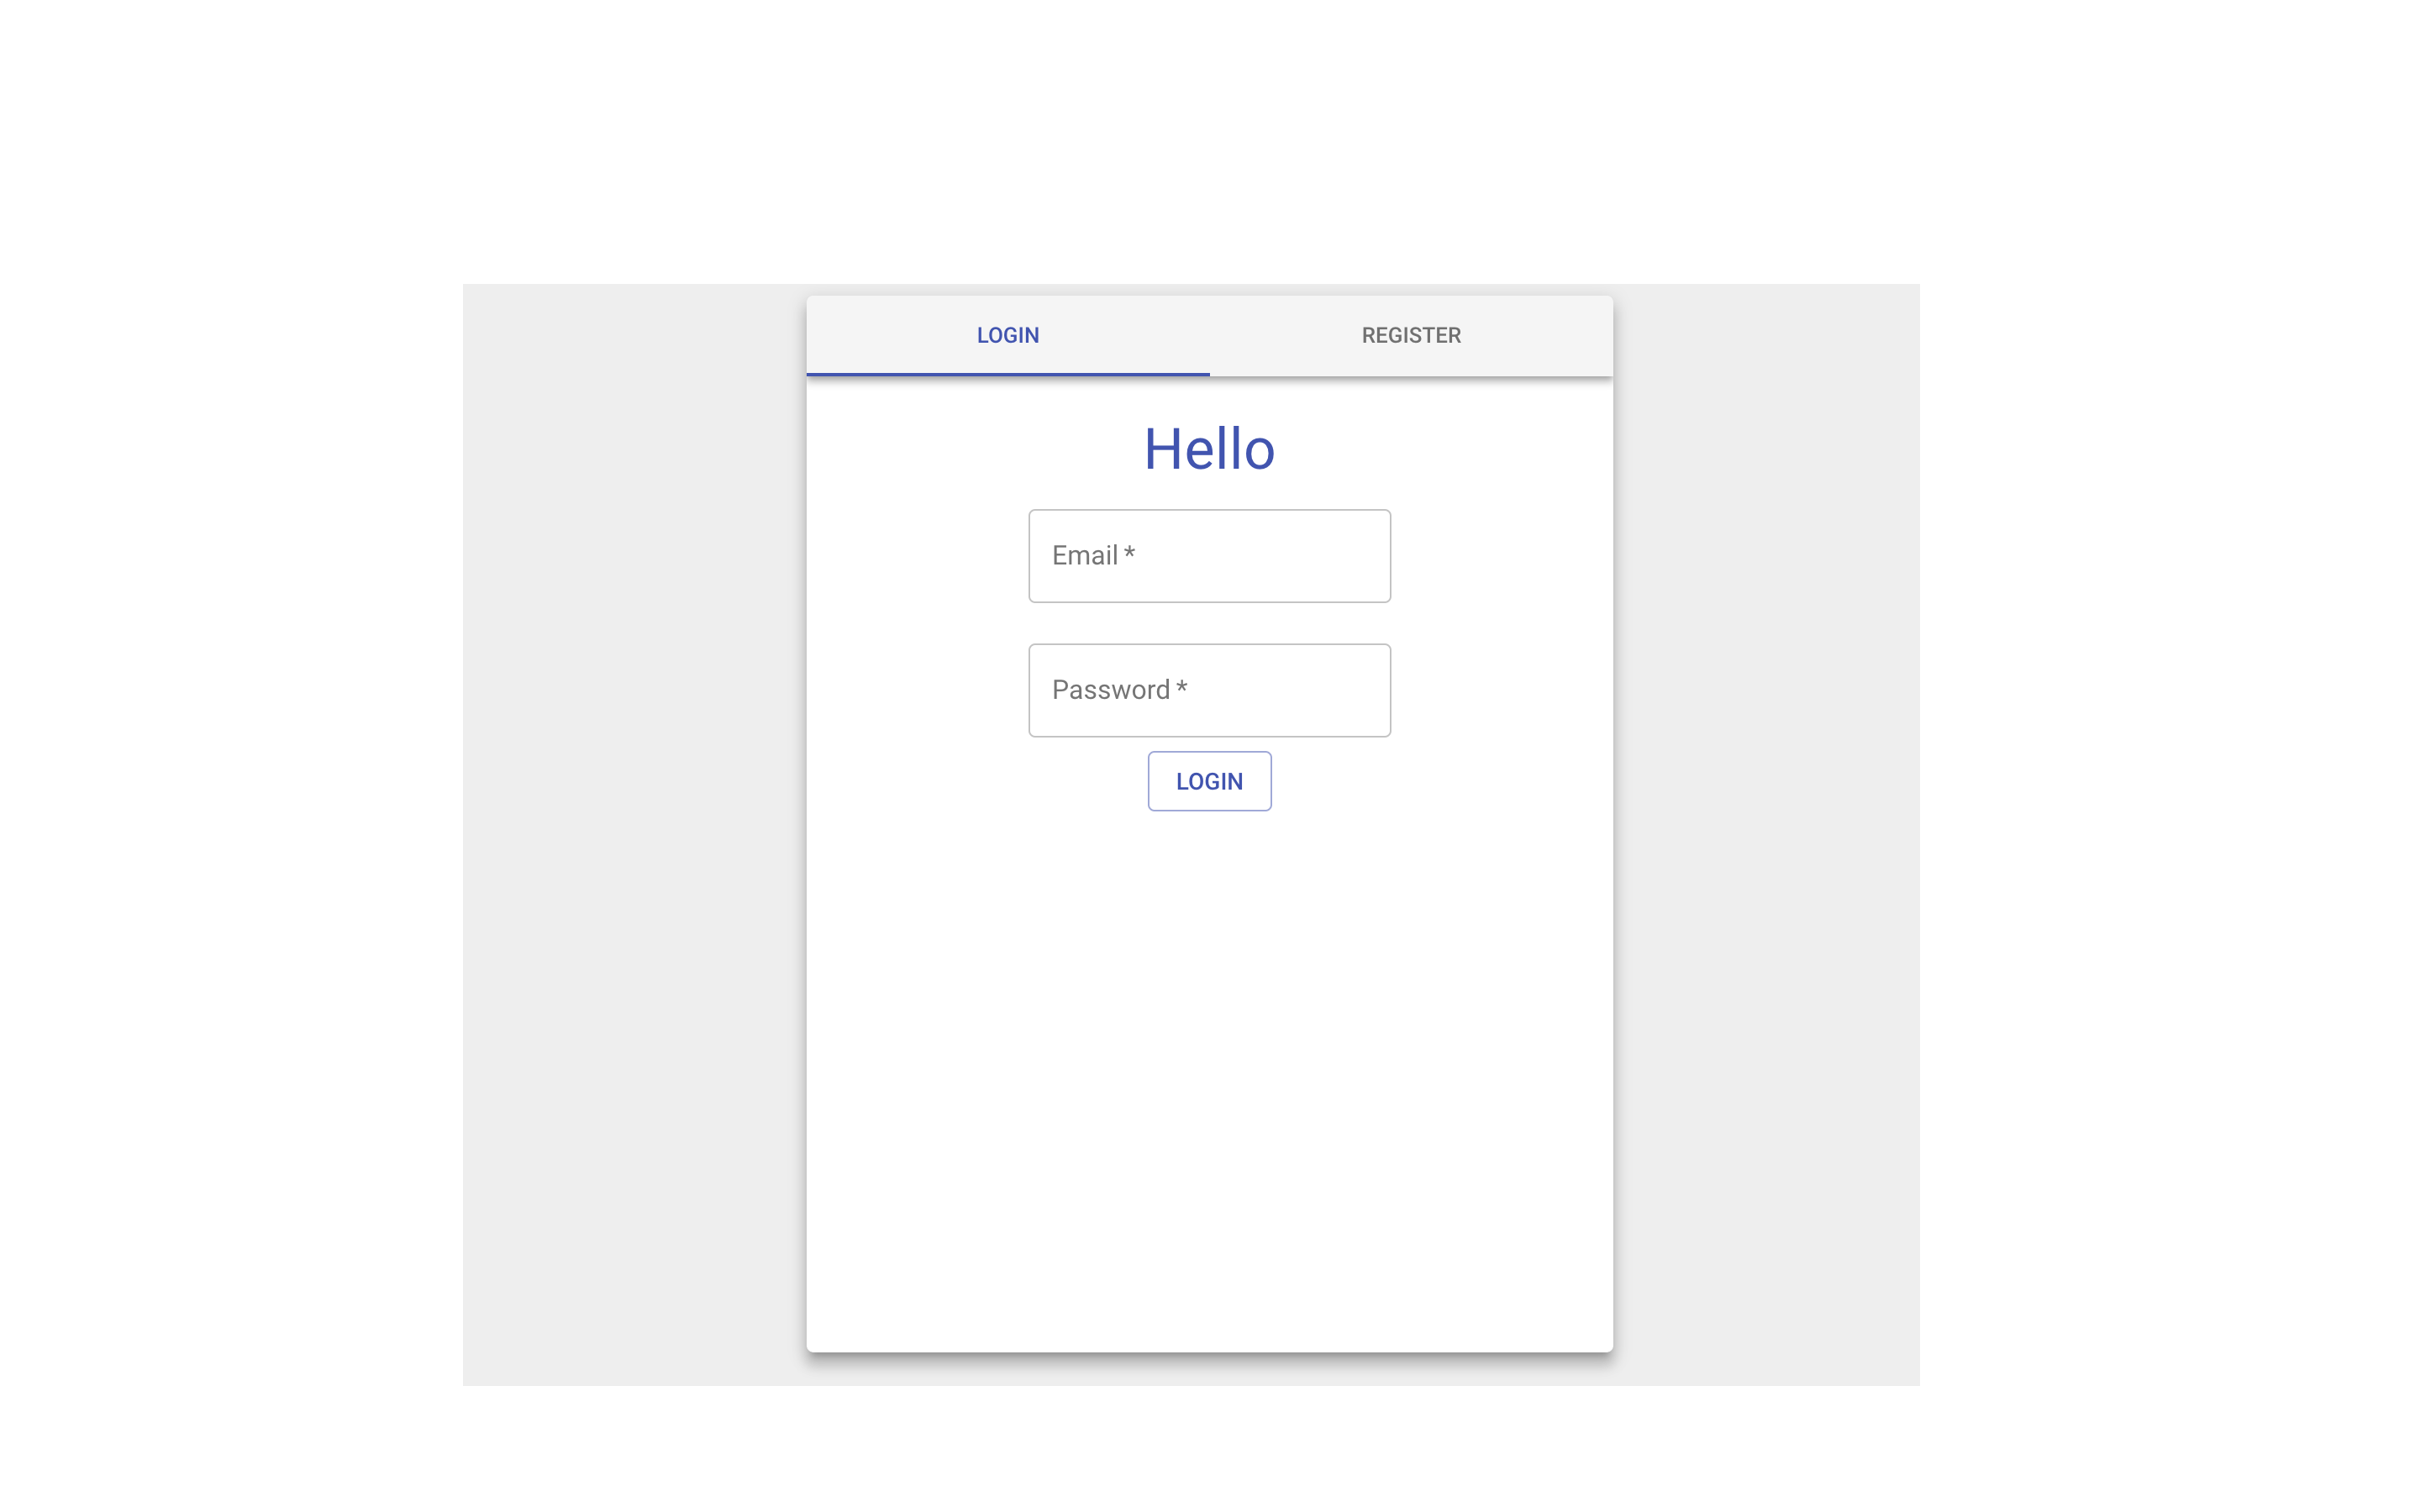
\includegraphics[width=\textwidth]{login.png}
         \caption{Login Screen}
     \end{figure}
     
    Click on \textbf{Register} tab to register as a new user. You should see this(Figure 8):
    
    \begin{figure}
        \centering
        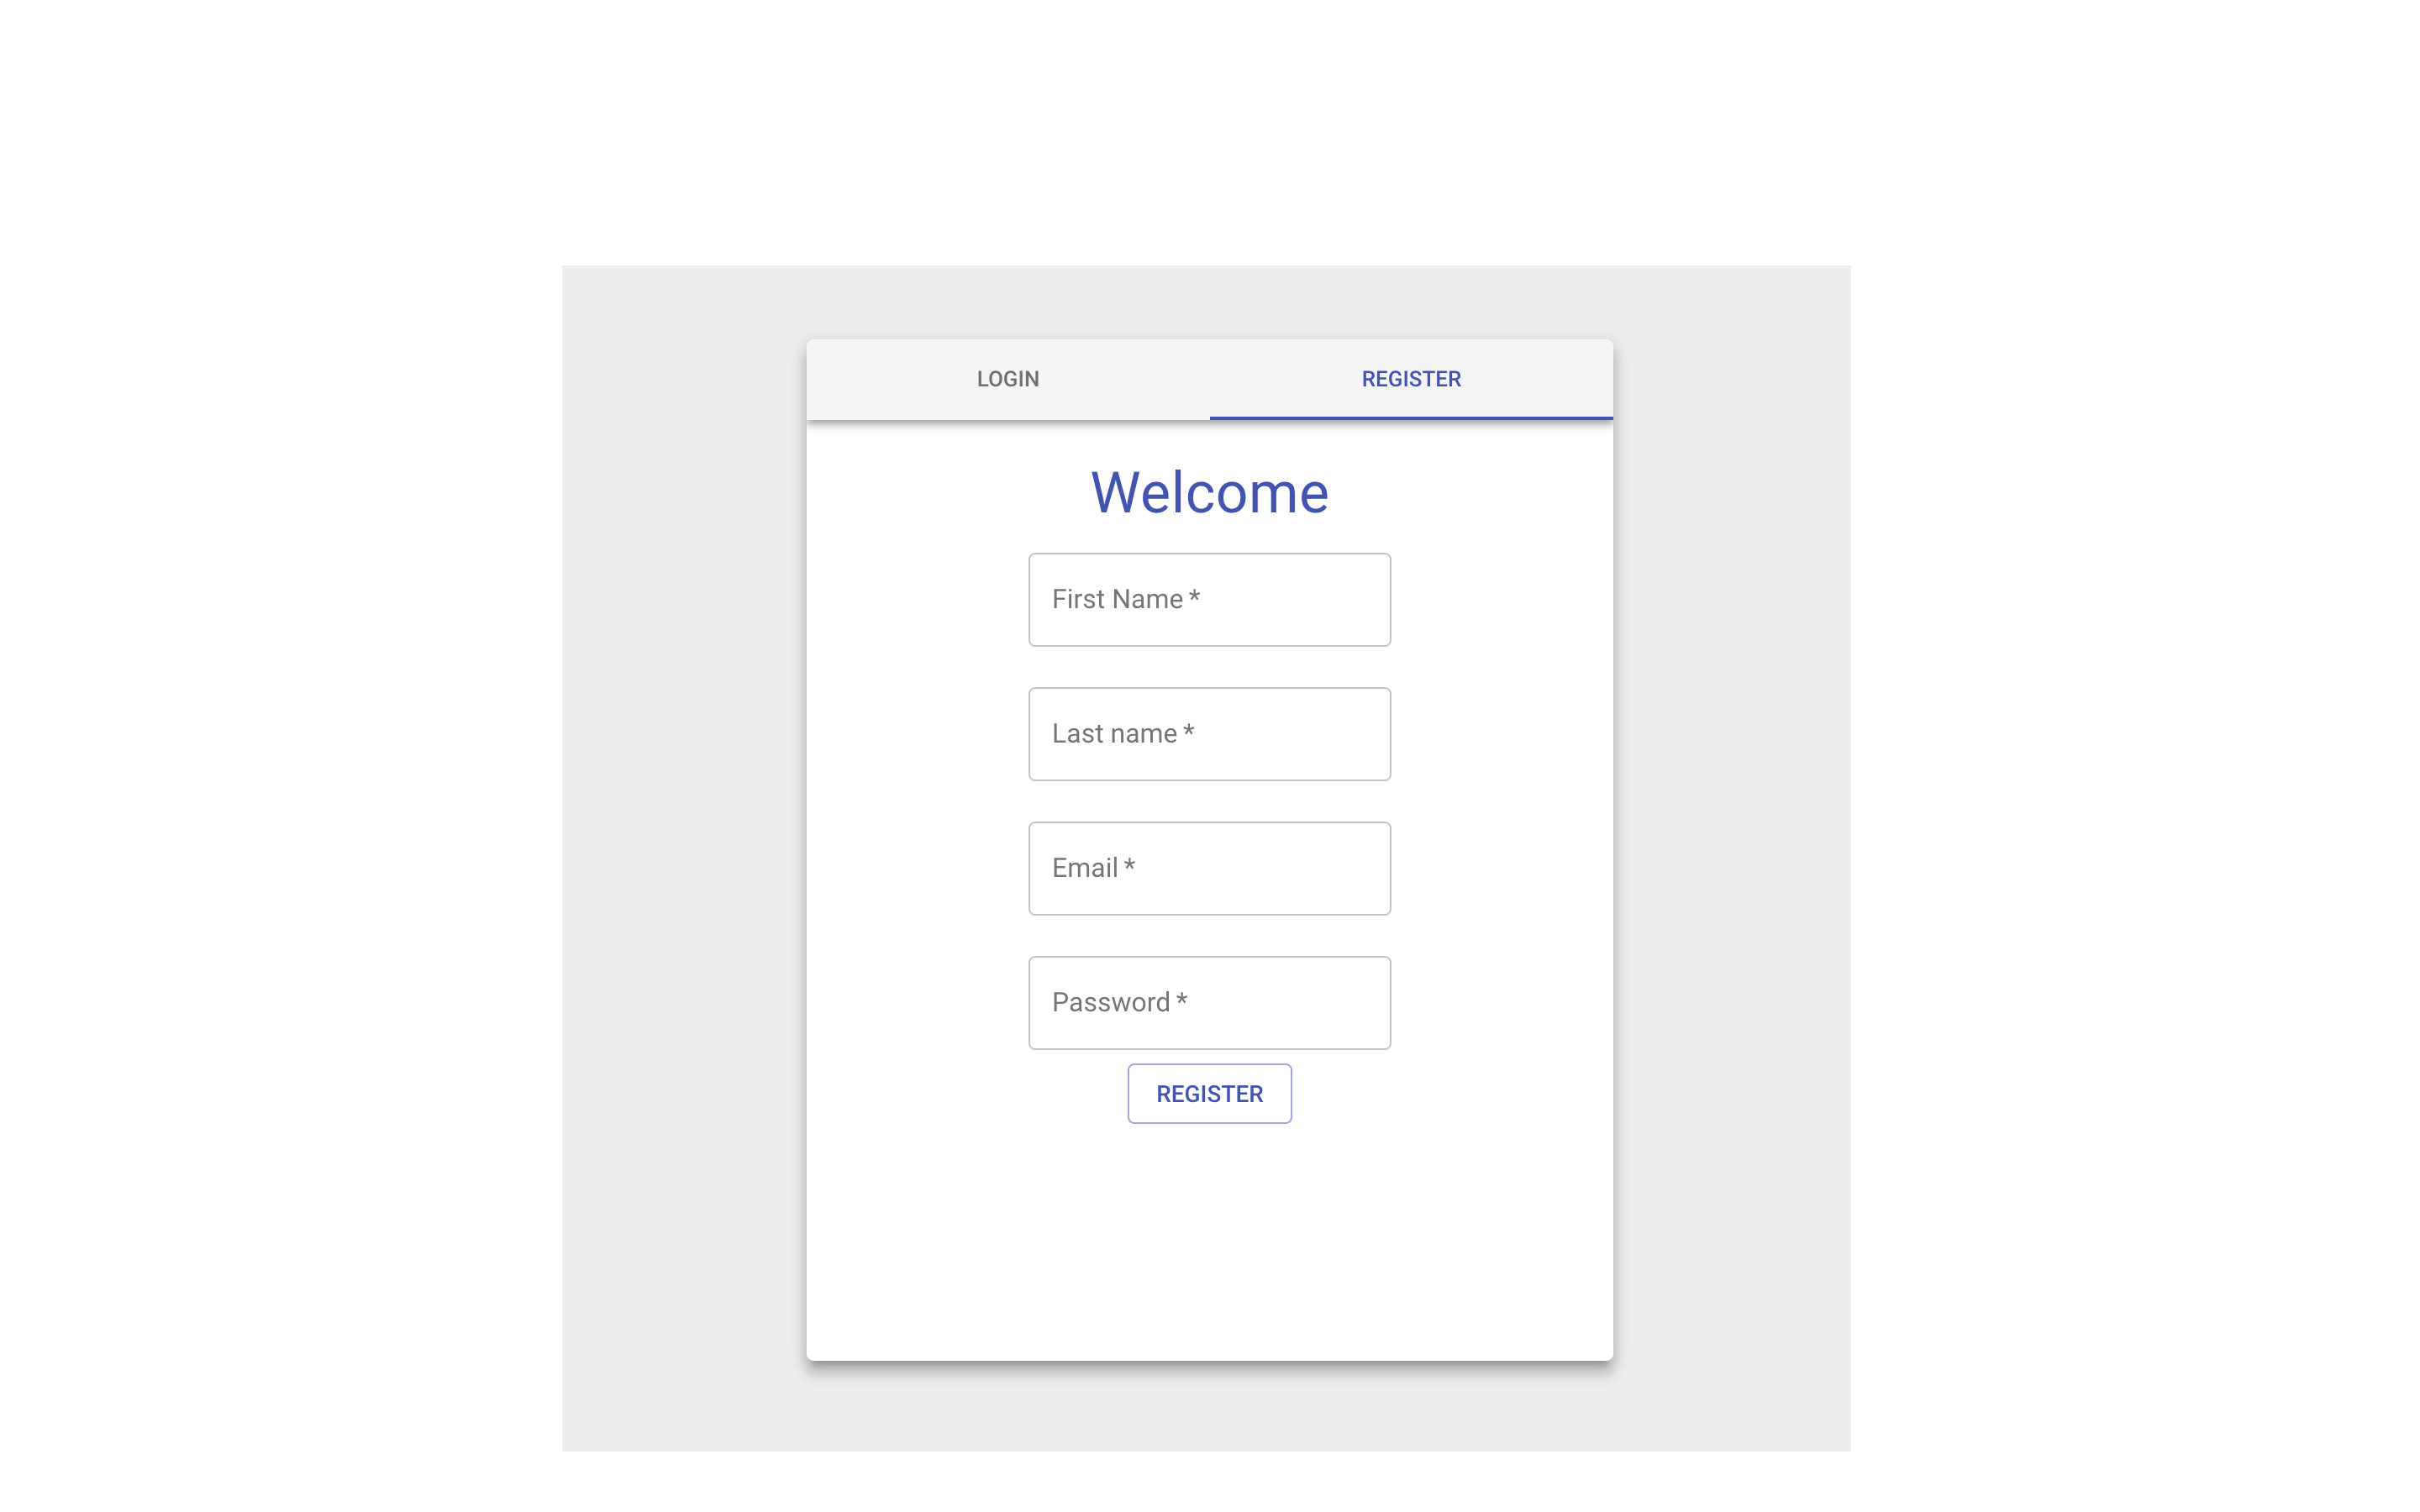
\includegraphics[width=10cm]{register.png}
         \caption{Register Screen}
        \end{figure}
    
    To register, fill in the following fields:
    \begin{itemize}
        \item First name
        \item Last name
        \item Email address
        \item Password 
    \end{itemize}
    
    Once the form is completed, click the \textbf{REGISTER} button at the bottom of the form. You should be directed to this page(Figure 9):
    
     \begin{figure}
        \centering
        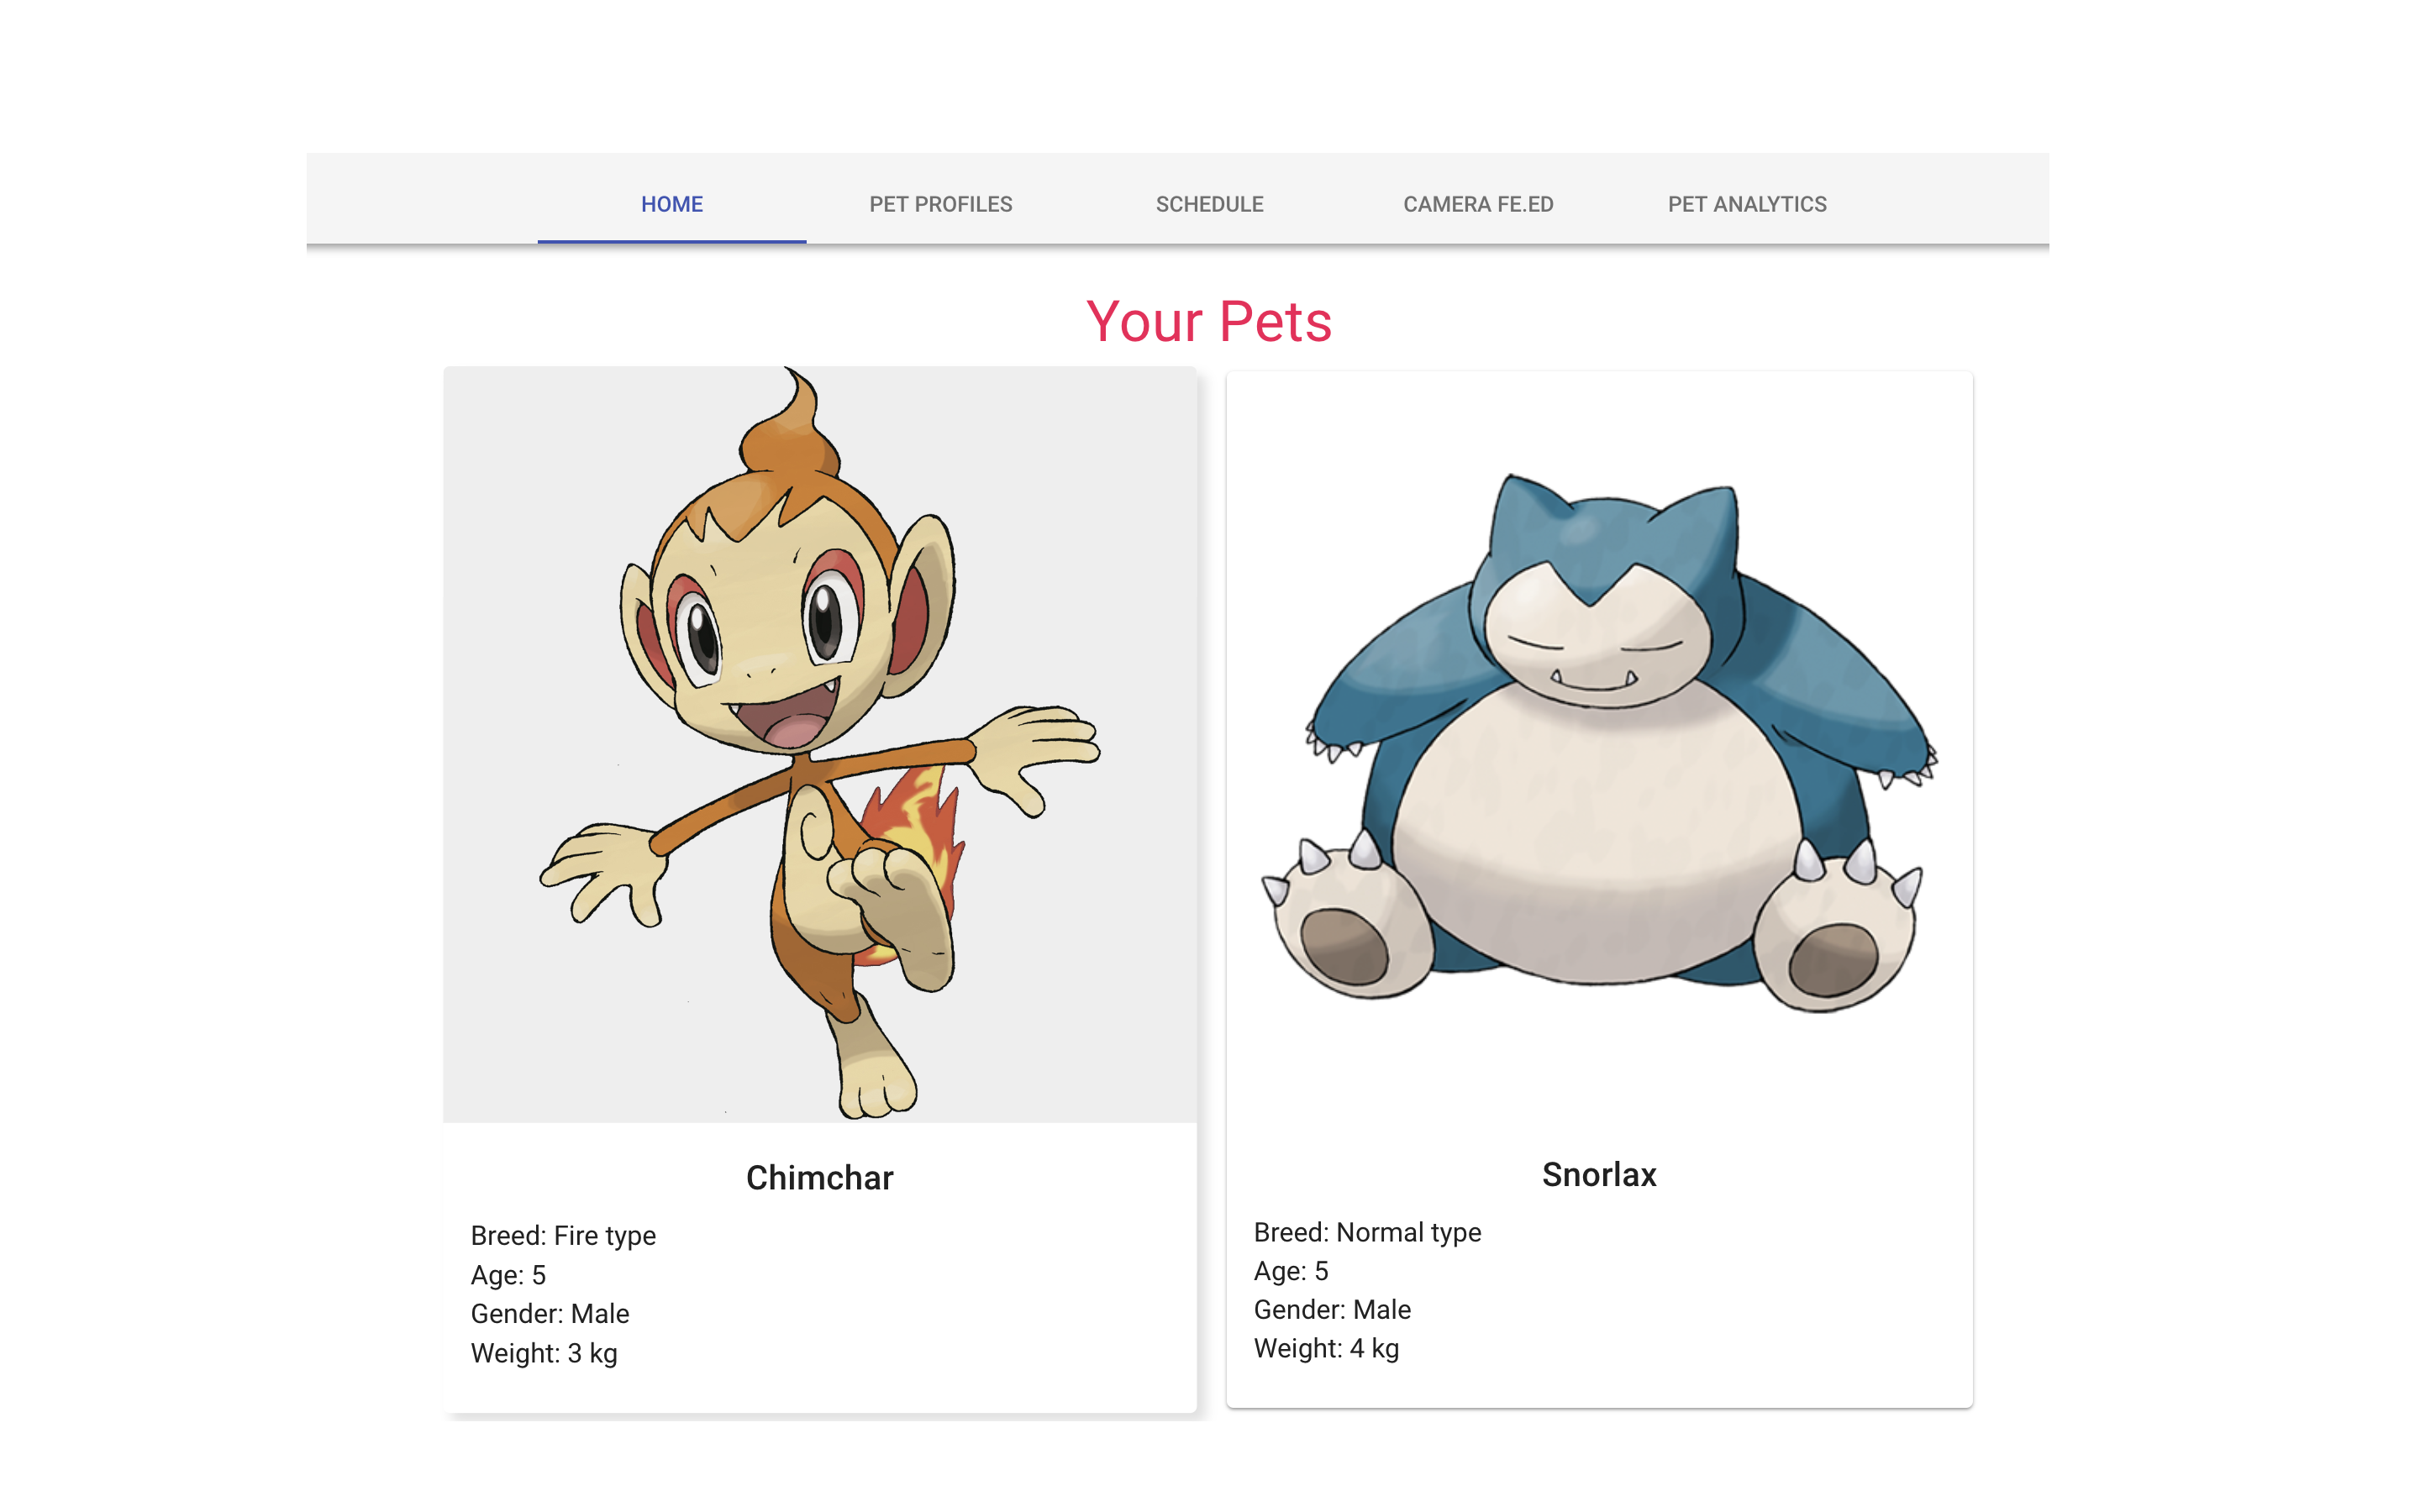
\includegraphics[width=10cm]{homepage.png}
         \caption{Homepage Screen}
        \end{figure}
    
    Next, you will need to create Pet Profiles. This is where you can give the application information about your pets. This allows the application to personalise it towards you and your pets for creating pet analytics (Section 3.5). Click on the Pet Profiles tab. You should see this(Figure 10)
    
    \begin{figure}
        \centering
        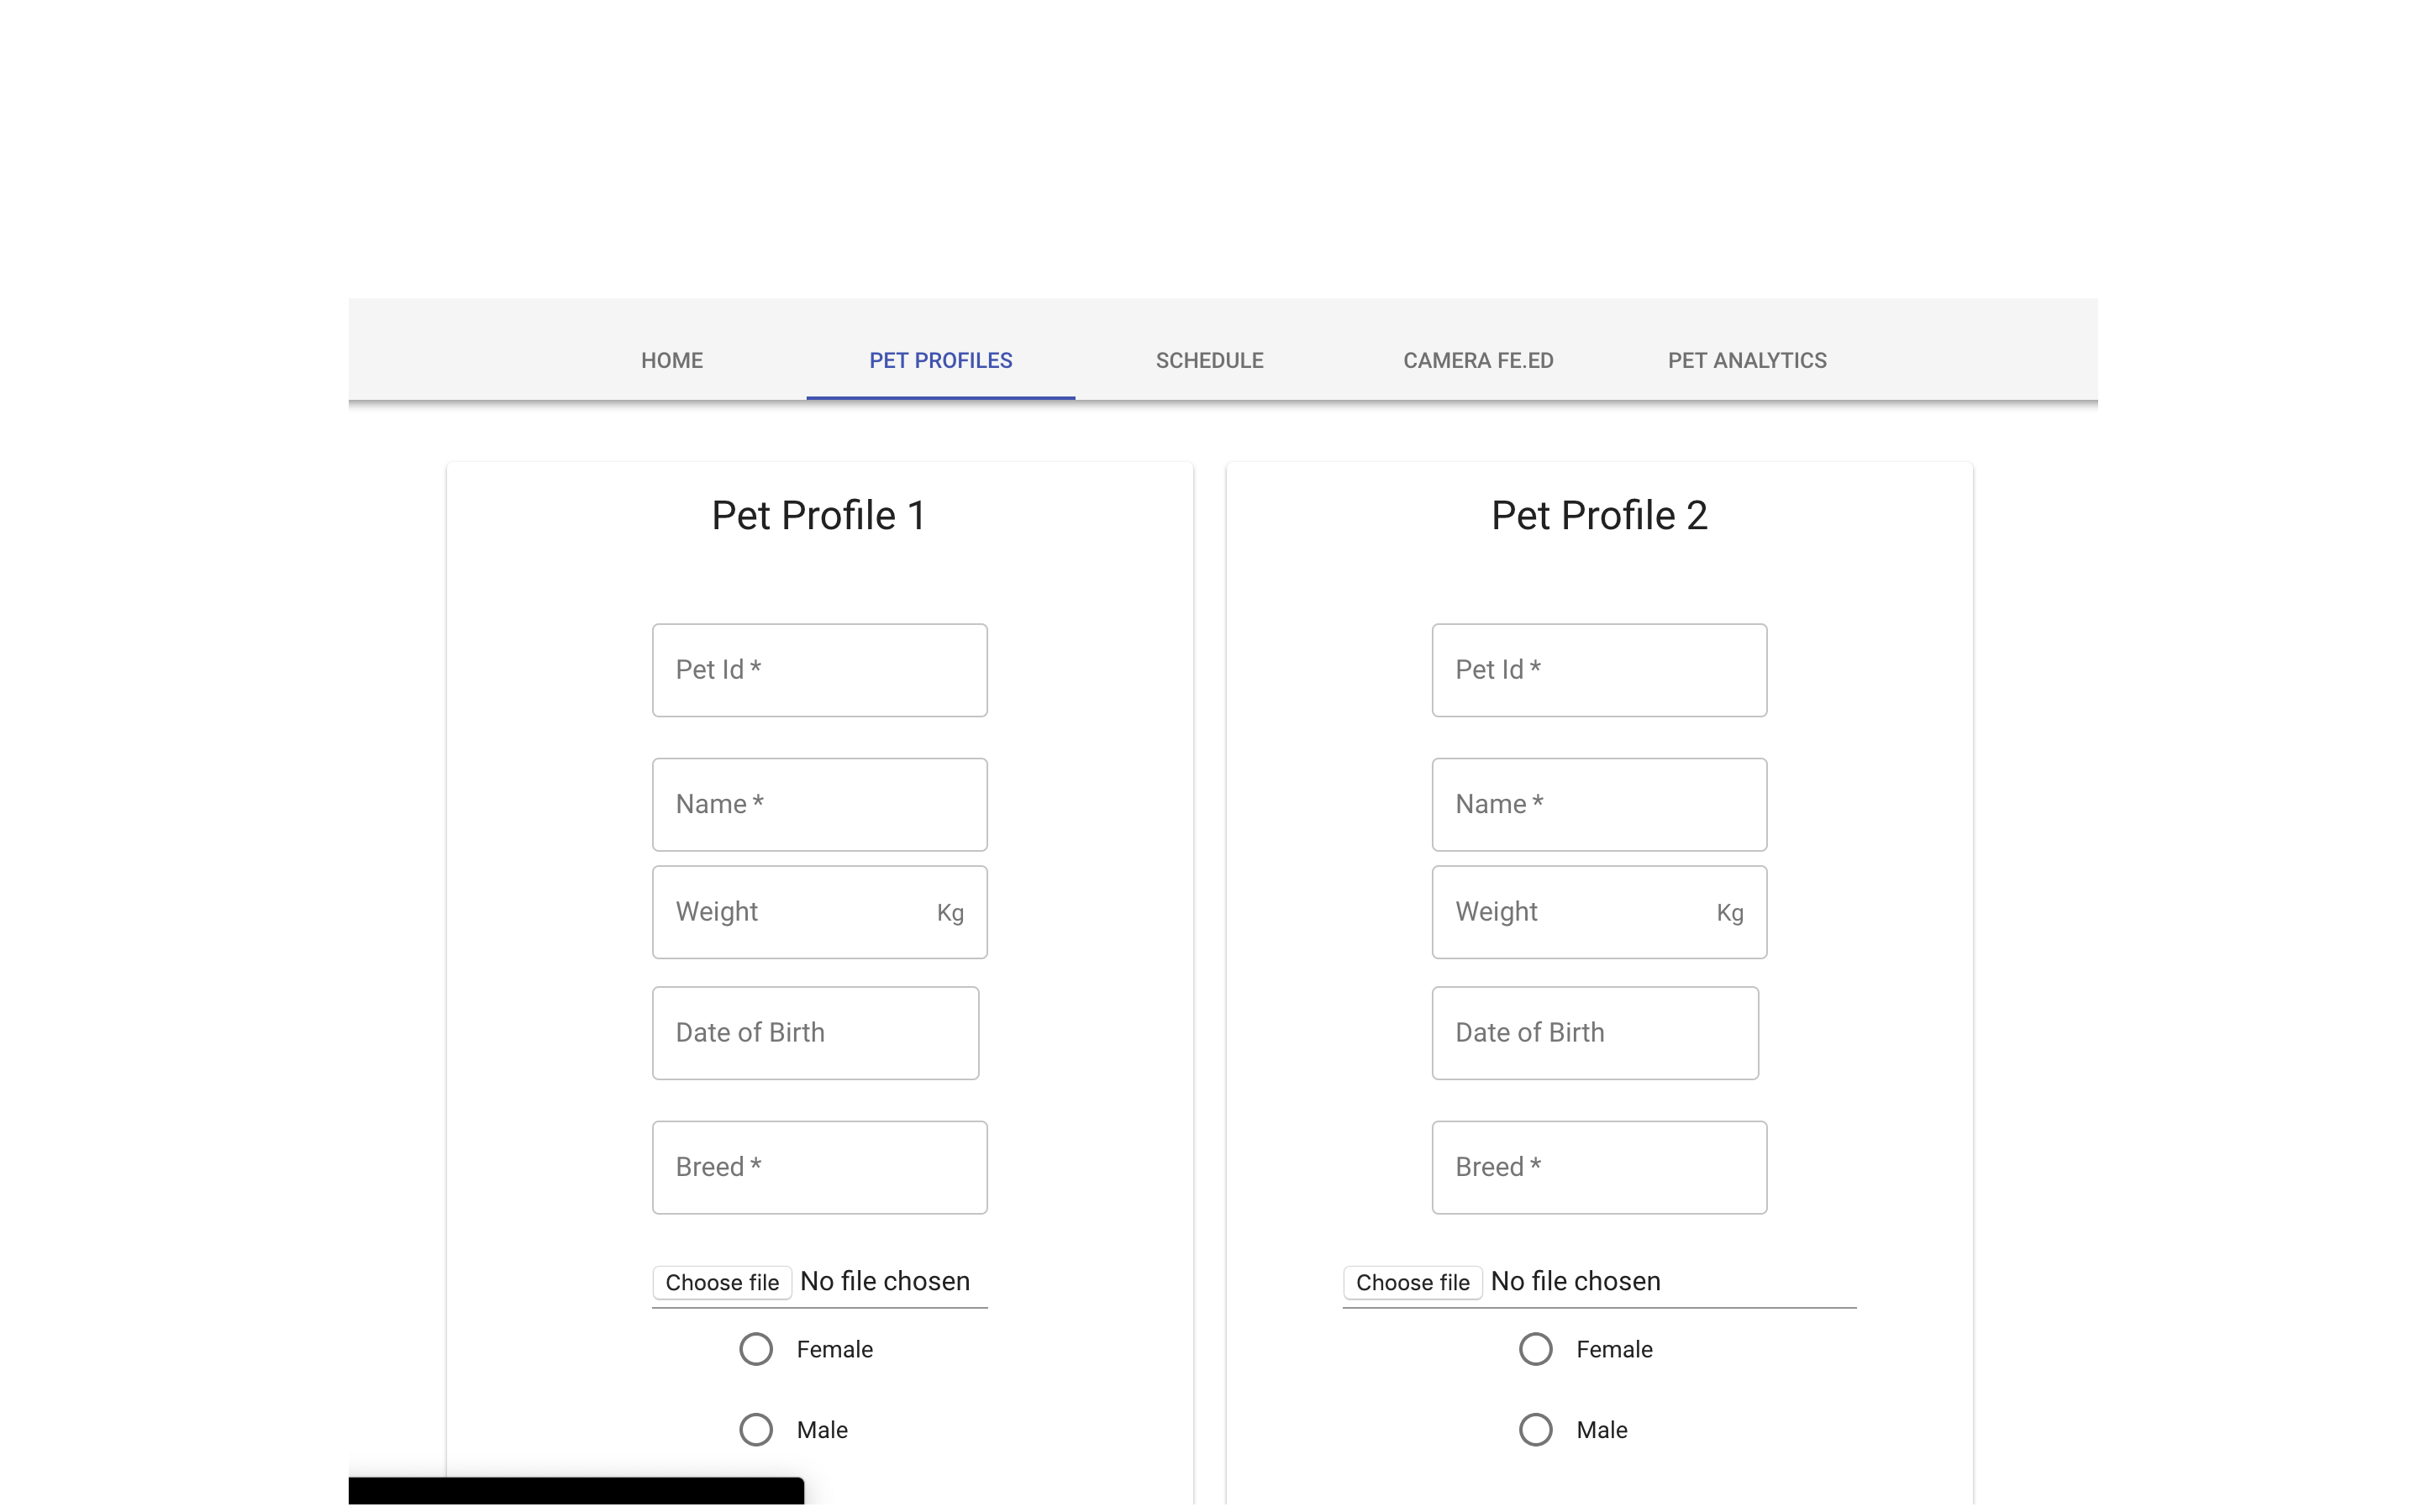
\includegraphics[width=10cm]{pets.png}
         \caption{Pet Profiles}
        \end{figure}
    
    After creating profiles for your pets, click the UPDATE  button. You should have successfully updated the pet profiles. You can check this by returning to the homepage (clicking on the HOME tab). You should see the dummy pets change to your own pets. 


\subsection{Making a Schedule}
Schedules are where you can set times to feed your pet. You can do this as one time only feed or a repeated one. Allowing you piece of mind that your pet will get their food, on time. This is where you can also specify the amount of food you want your pet to be fed. To create a schedule to feed your pets, click on the “SCHEDULE” tab. (Figure 11)

 \begin{figure}
        \centering
        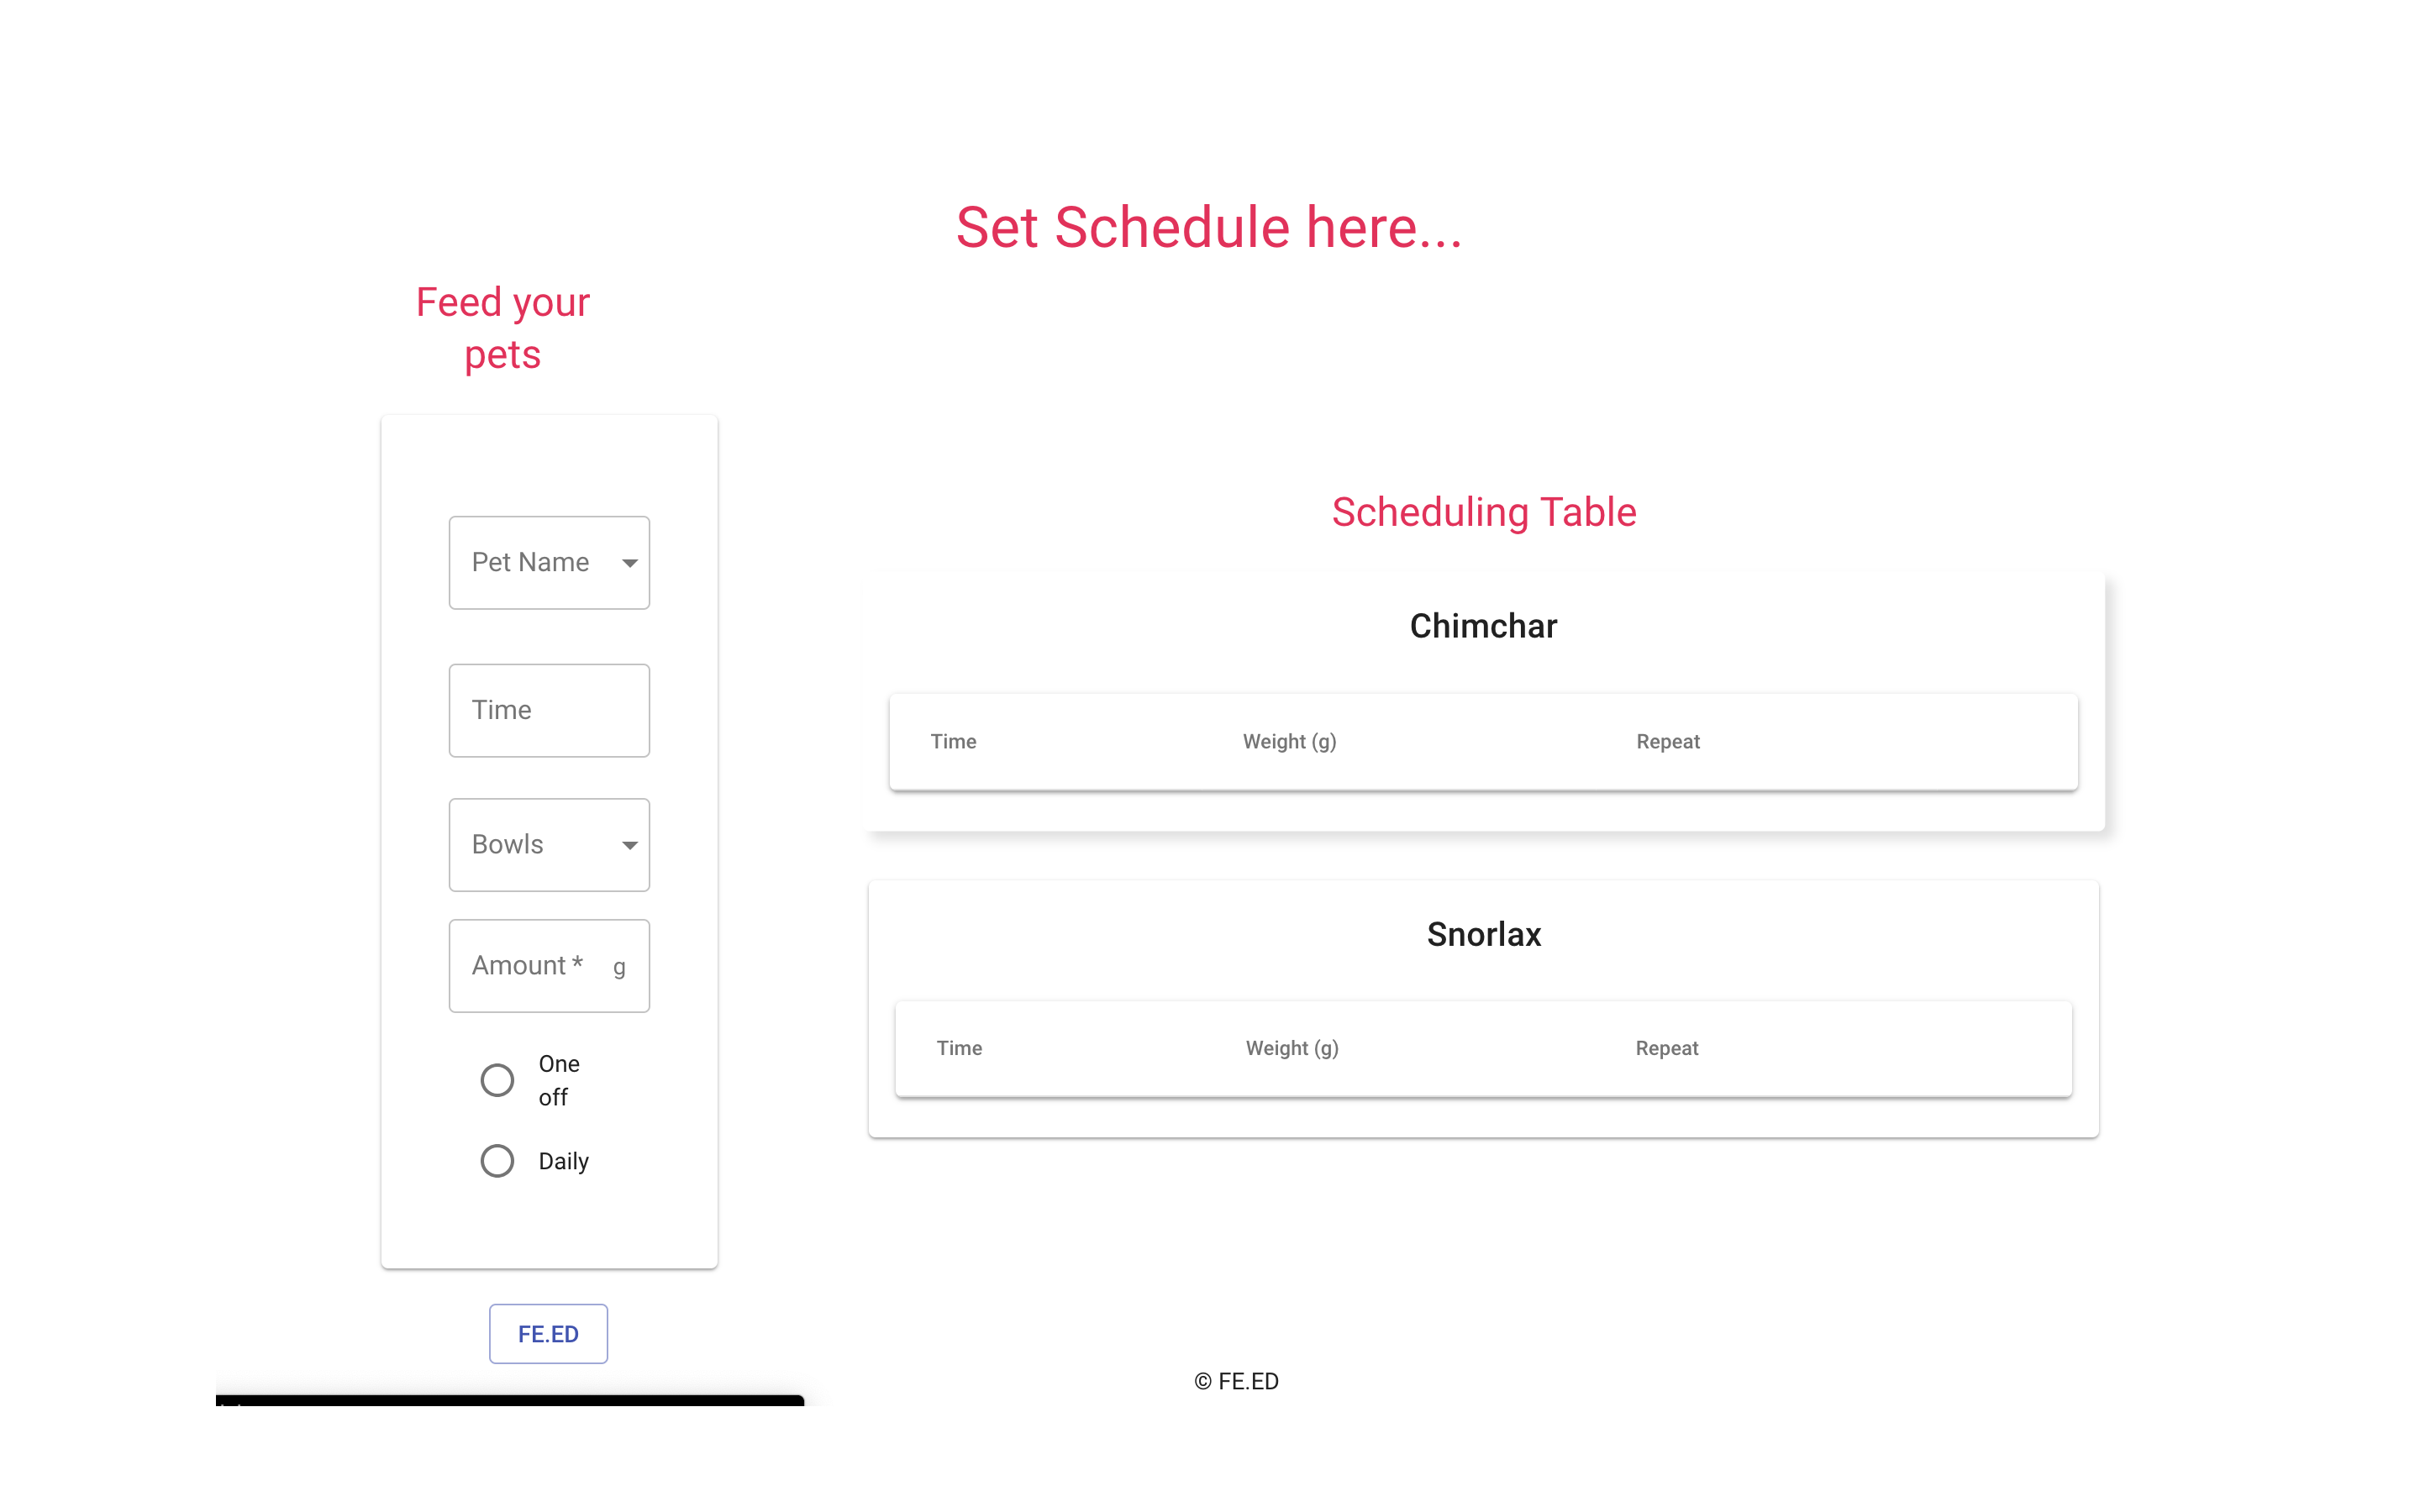
\includegraphics[width=14cm]{schedule.png}
         \caption{Schedule}
        \end{figure}

Fill in the form under “Feed your pets” . You need to fill in the following fields:
\begin{itemize}
\item Pet Name 
\item Time 
\item Bowl
\item Weight of food per serving (measured in grams)
\item One of feed or Daily (if you would like it repeated every day)
\end{itemize}

Click “FE.ED” to set the schedule.Once set, the 3 most recent schedules are shown on the app for each pet. (Figure 12)

 \begin{figure}
        \centering
        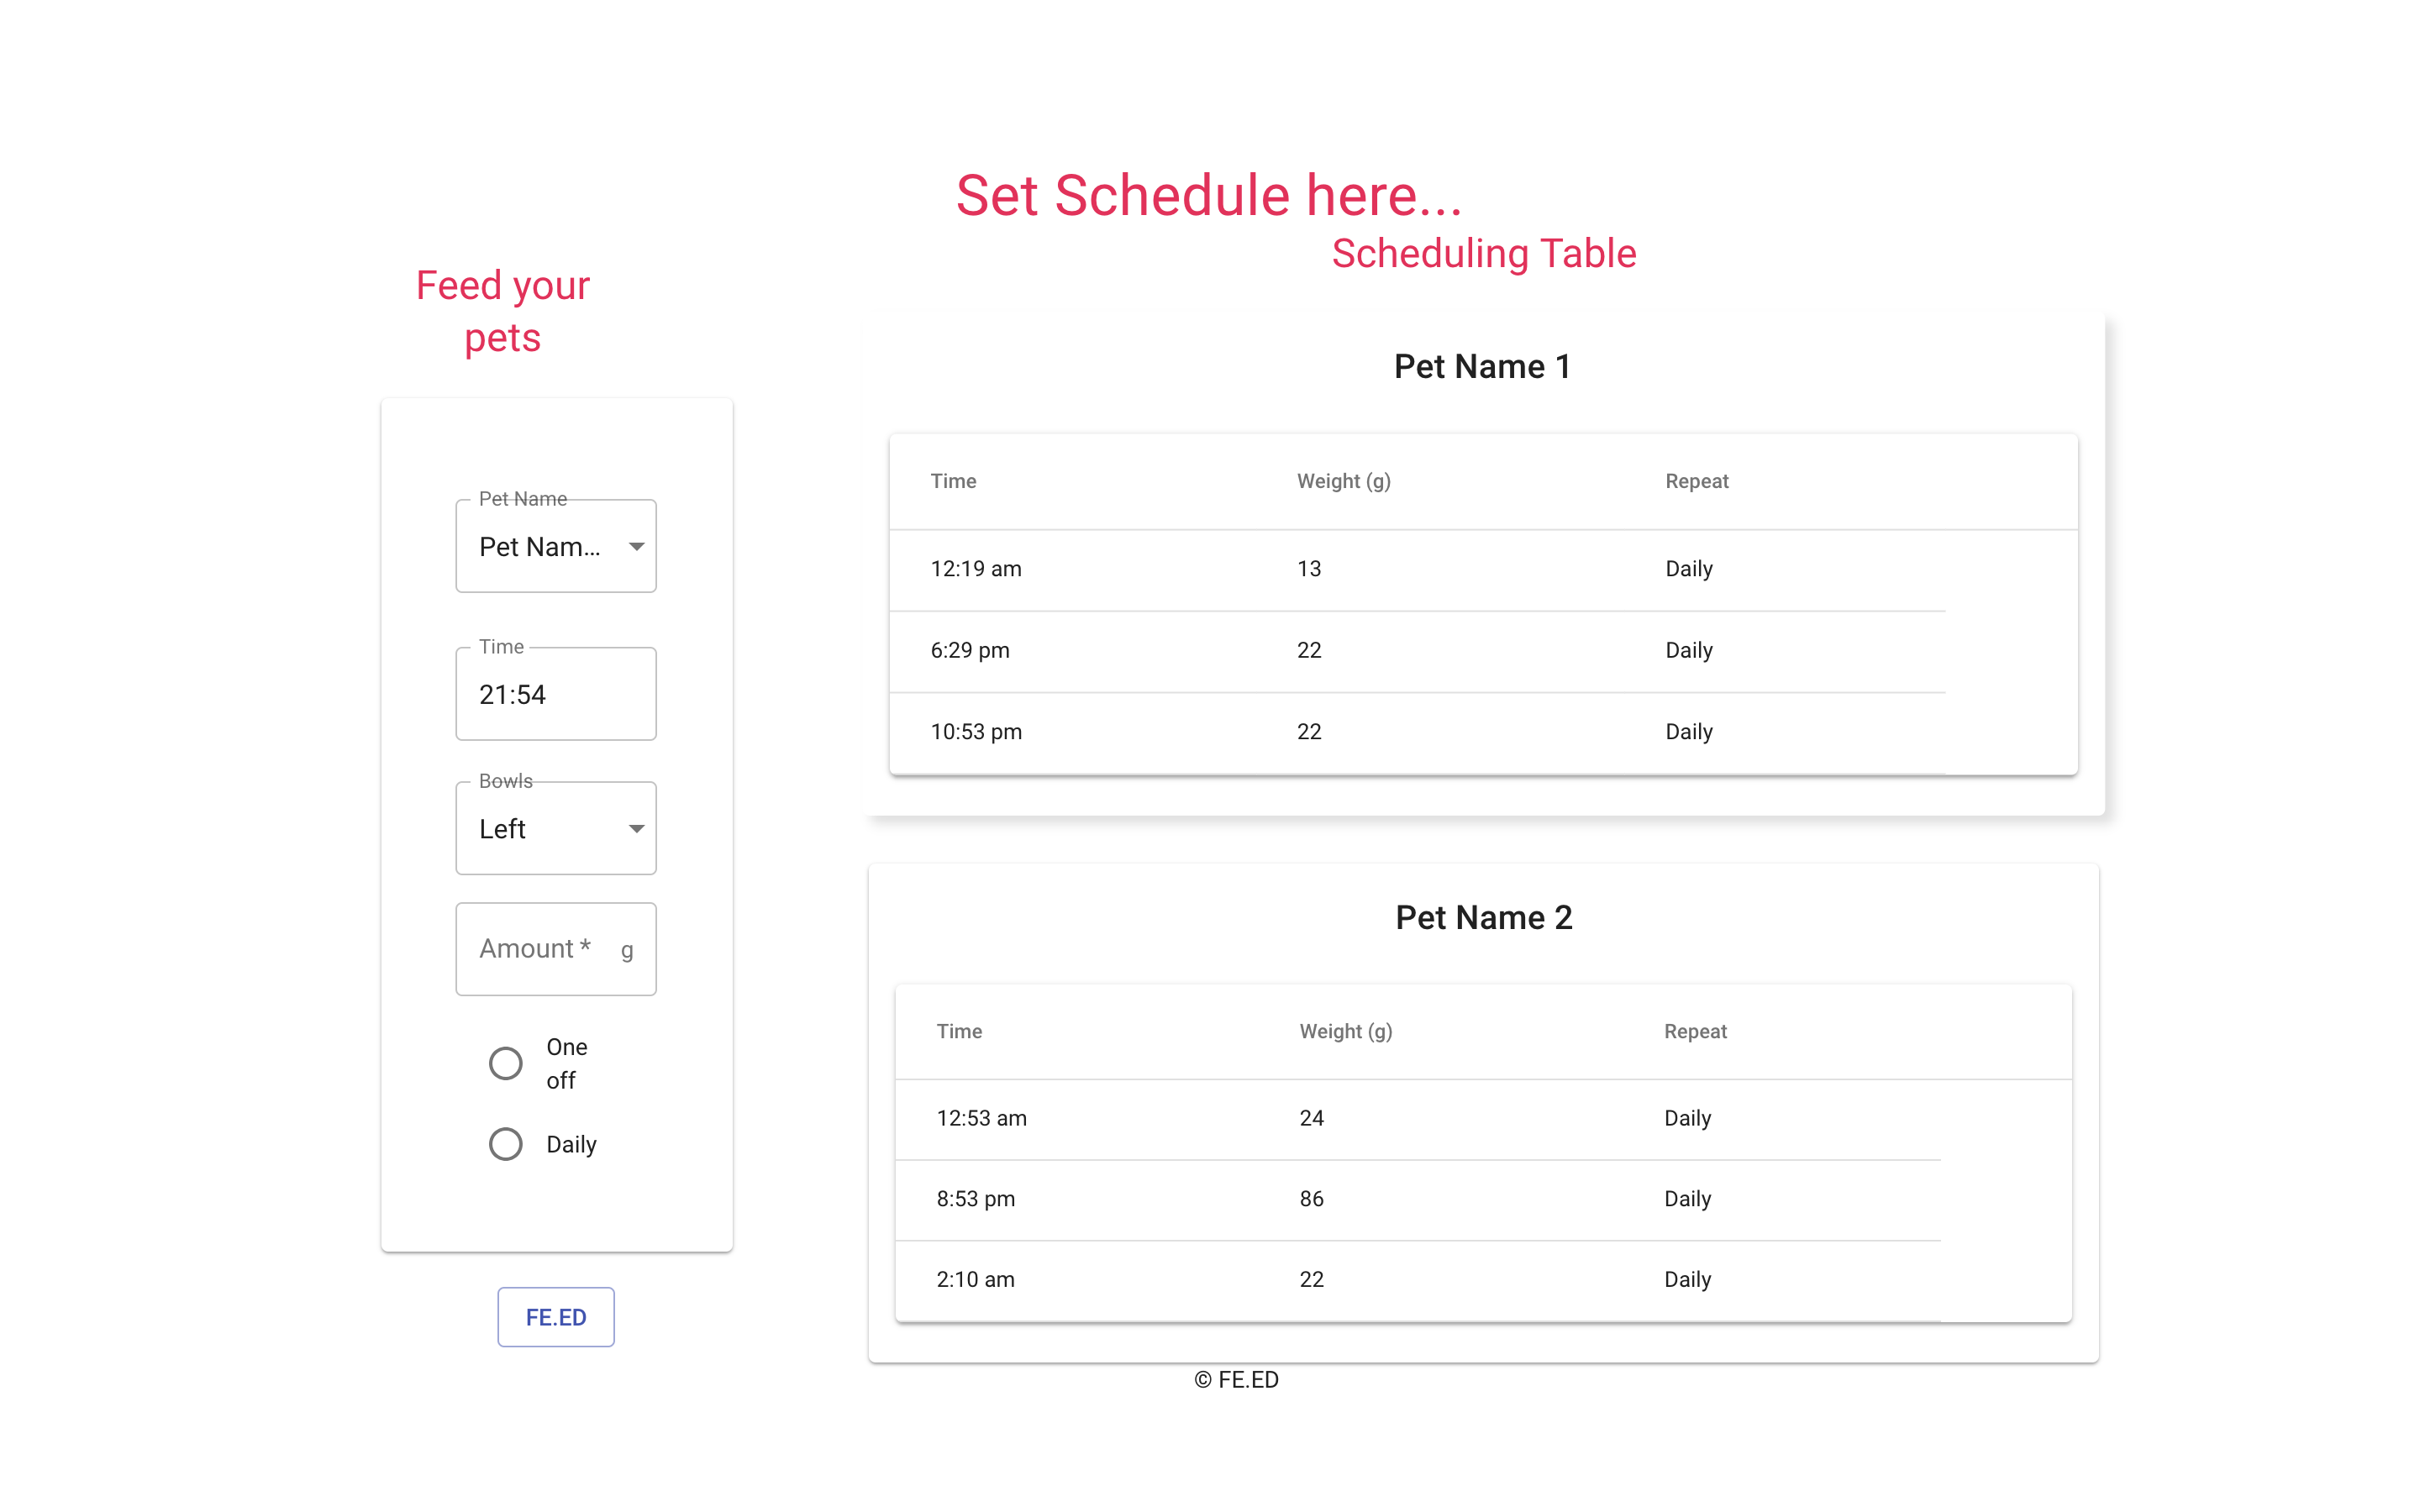
\includegraphics[width=14cm]{fill.png}
         \caption{Filled Schedule}
        \end{figure}



\subsection{Other uses for the Application}
    
\subsubsection{Camera FE.ED}
The live camera feed allows you to see your pets on the web application. When the robot dispenses food, the camera turns on allowing you to see your pet. There are also Left and Right buttons which give you control of the camera and allow you to rotate the camera so you can have better visibility of your pet depending on where they are. The pet feeder comes with the camera set up at the correct angle to view your pets as they eat their food, however the user is free to adjust the angle as they see fit.(Figure 13)

 \begin{figure}
        \centering
        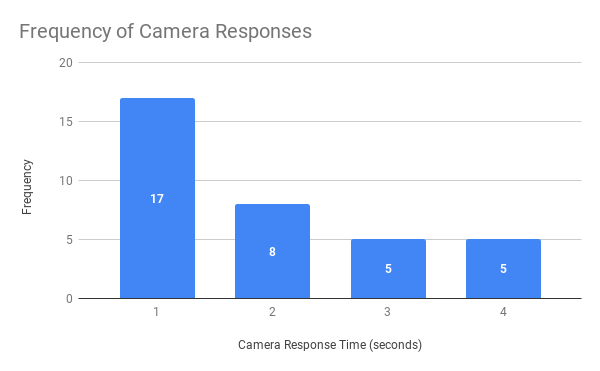
\includegraphics[width=14cm]{camera.png}
         \caption{Camera FE.ED}
        \end{figure}


        
\subsubsection{Pet Analytics}
The pet analytics page displays graphs showing the quantity of food your pet has eaten. This allows you to make sure that your pet is eating the right amount of food. The graph also displays a prediction based on current eating trends, so you can plan your pets meals in advance. (Figure 14)

 \begin{figure}
        \centering
        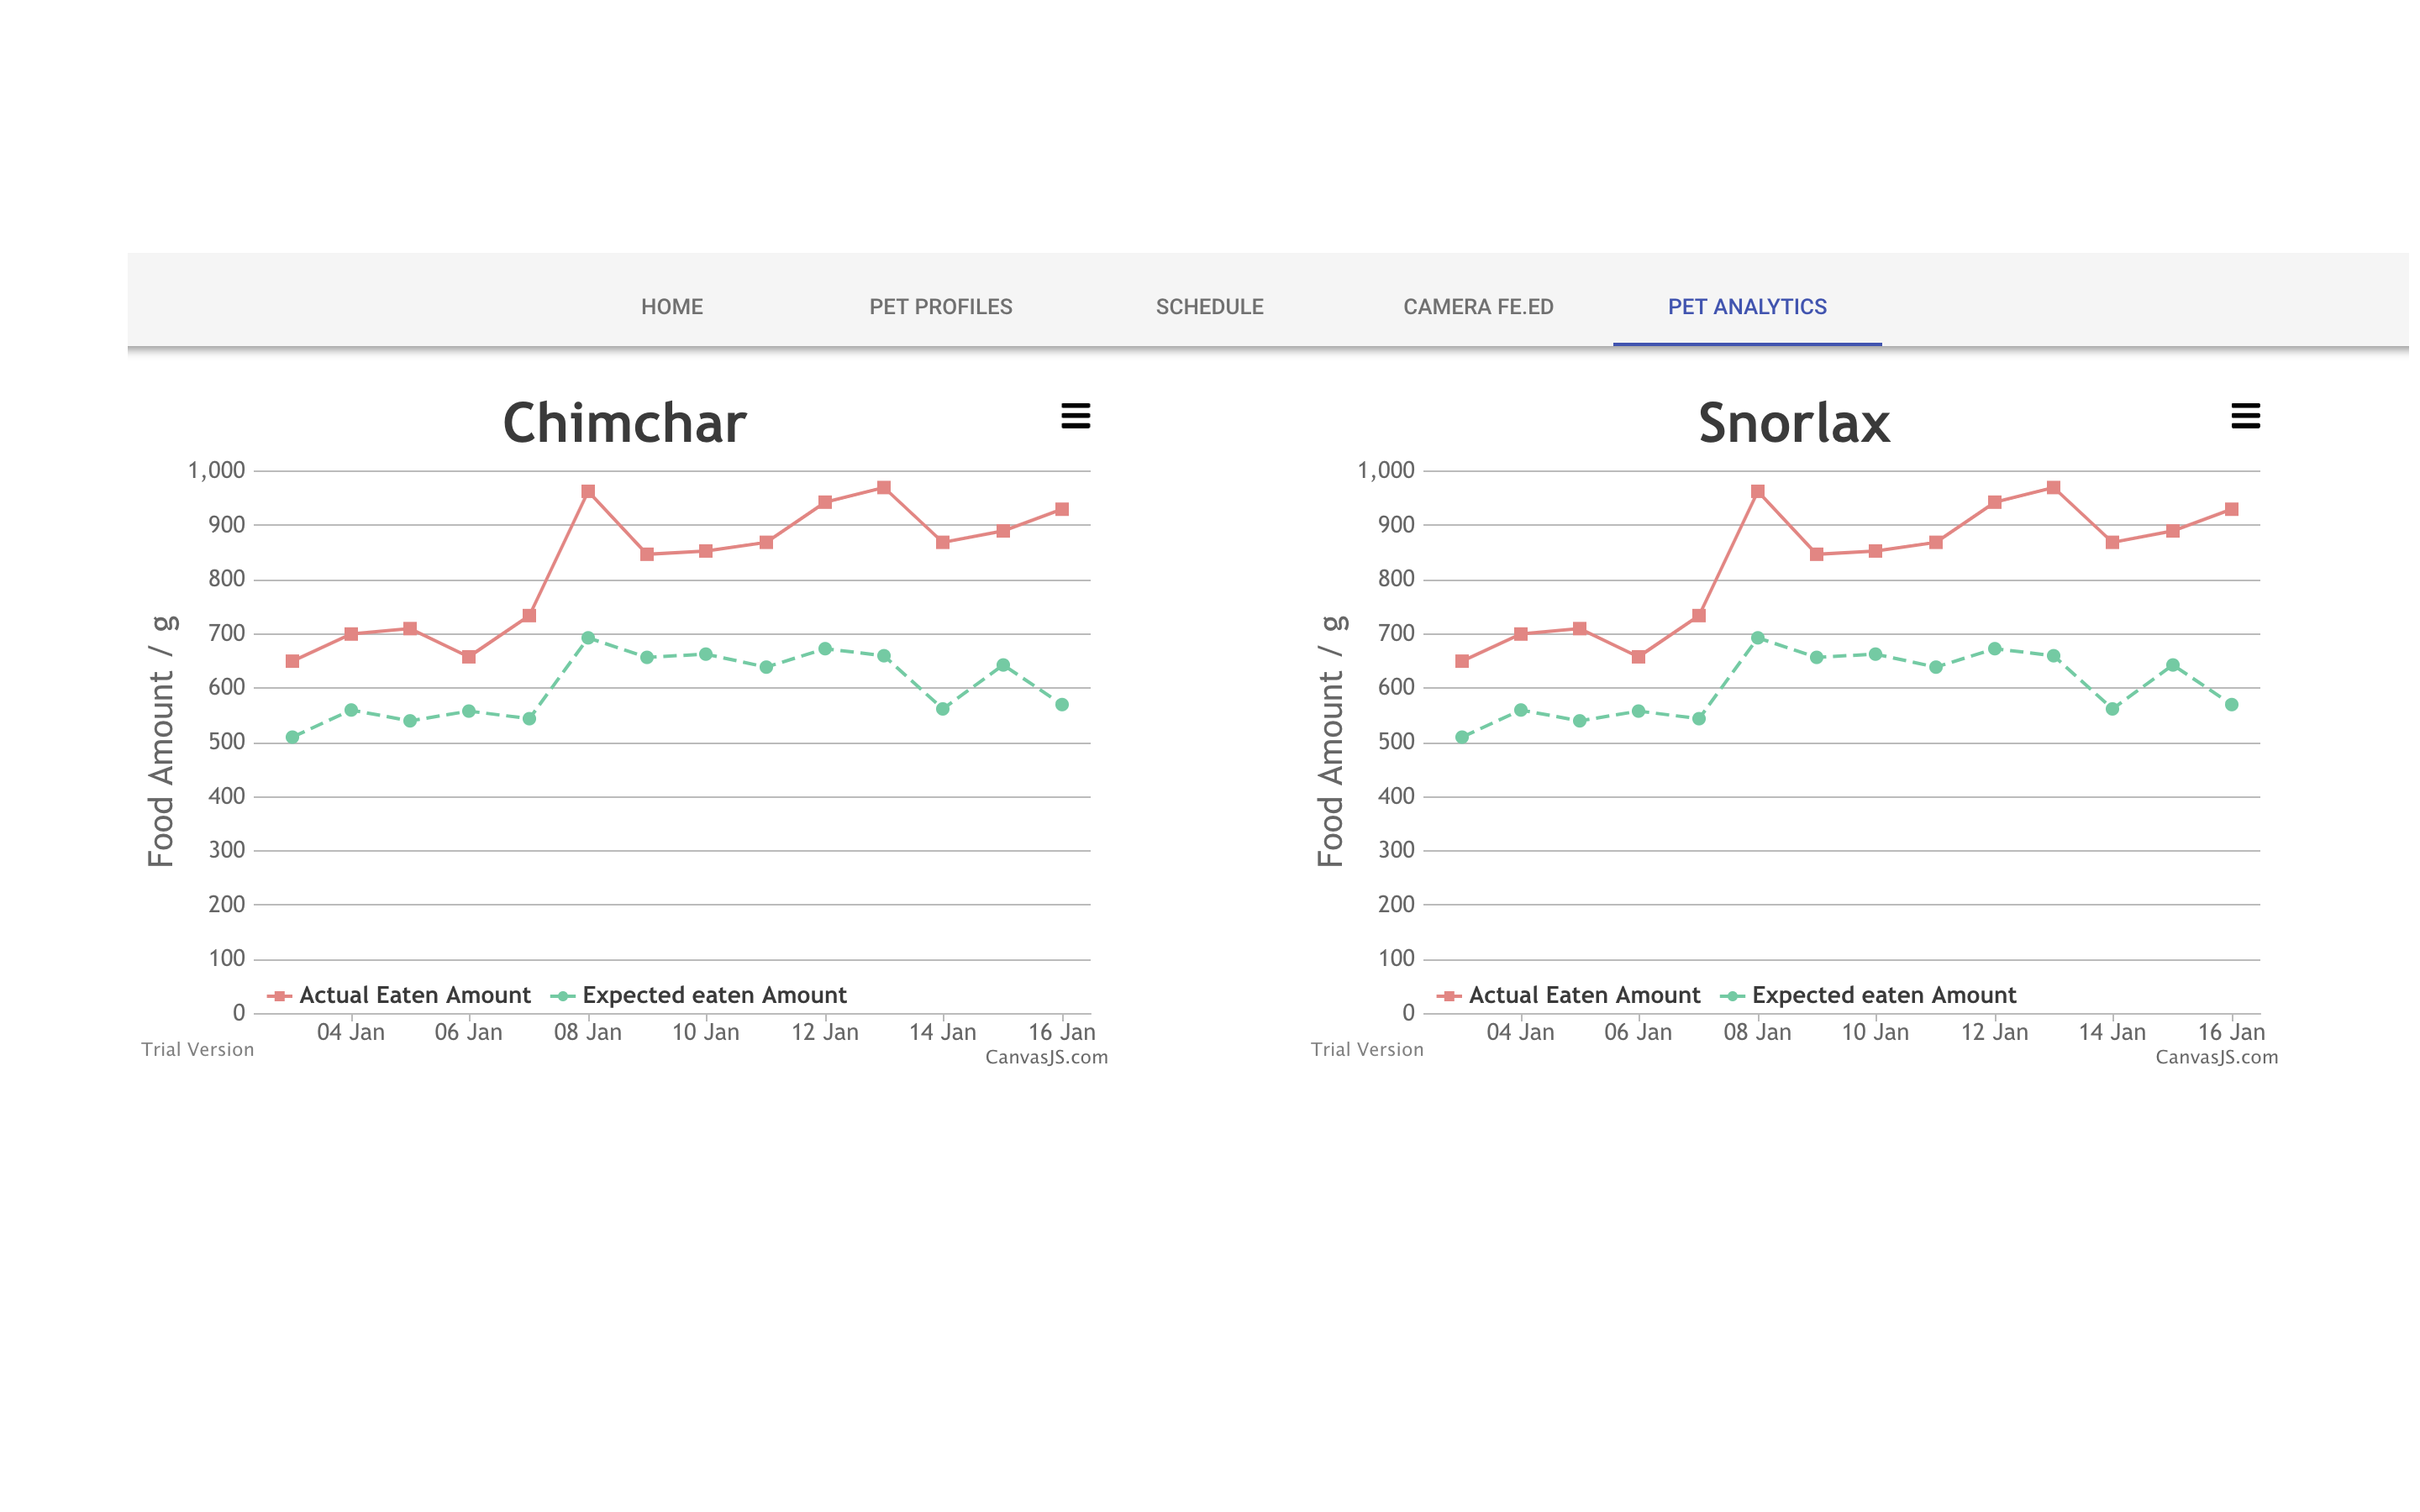
\includegraphics[width=14cm]{data.png}
         \caption{Pet Analytics}
        \end{figure}


\subsection{Cleaning the containers}
Over time, dust and dirt can build up throughout the machine. It’s therefore a good idea to occasionally clean out the machine. This can be done by gently removing the cover from the robot and wiping it down with a damp cloth. Make sure the robot is turned off when doing this.
    
    